\documentclass[a4paper,10pt,twoside]{article}

\usepackage[top=1in, bottom=1in, left=1in, right=1in]{geometry}
\usepackage[utf8]{inputenc}

\usepackage{fancyhdr}
\usepackage{graphicx}

%\usepackage{lastpage}


%%%%%%%%%% Configuración de Fancyhdr - Inicio %%%%%%%%%%
\pagestyle{fancy}
\thispagestyle{fancy}
\lhead{TP2, Sistemas Operativos}
\renewcommand{\footrulewidth}{0.4pt}
\cfoot{\thepage /\pageref{LastPage}}

\fancypagestyle{caratula} {
   \fancyhf{}
   \cfoot{\thepage /\pageref{LastPage}}
   \renewcommand{\headrulewidth}{0pt}
   \renewcommand{\footrulewidth}{0pt}
}

%%%%%%%%%% Macros de tikz - Fin %%%%%%%%%%


\begin{document}


%%%%%%%%%%%%%%%%%%%%%%%%%%%%%%%%%%%%%%%%%%%%%%%%%%%%%%%%%%%%%%%%%%%%%%%%%%%%%%%
%% Carátula                                                                  %%
%%%%%%%%%%%%%%%%%%%%%%%%%%%%%%%%%%%%%%%%%%%%%%%%%%%%%%%%%%%%%%%%%%%%%%%%%%%%%%%


\thispagestyle{caratula}

\begin{center}


\includegraphics[height=2cm]{DC.png} 
\hfill

\includegraphics[height=2cm]{UBA.jpg} 

\vspace{2cm}

Departamento de Computación,\\
Facultad de Ciencias Exactas y Naturales,\\
Universidad de Buenos Aires

\vspace{4cm}

\begin{Huge}
TP2 - Pthreads
\end{Huge}

\vspace{0.5cm}

\begin{Large}
Sistemas Operativos
\end{Large}

\vspace{1cm}

Primer Cuatrimestre de 2015

\vspace{4cm}

\vspace{0.5cm}

\begin{tabular}{|c|c|c|}
\hline
Apellido y Nombre & LU & E-mail\\
\hline
Cisneros Rodrigo		& 920/10 & rodricis@hotmail.com\\
Rodr\'iguez, Agust\'in	& 120/10 & agustinrodriguez90@hotmail.com\\
Tripodi, Guido			& 843/10 & guido.tripodi@hotmail.com\\
\hline
\end{tabular}

\end{center}

\newpage


%%%%%%%%%%%%%%%%%%%%%%%%%%%%%%%%%%%%%%%%%%%%%%%%%%%%%%%%%%%%%%%%%%%%%%%%%%%%%%%
%% Índice                                                                    %%
%%%%%%%%%%%%%%%%%%%%%%%%%%%%%%%%%%%%%%%%%%%%%%%%%%%%%%%%%%%%%%%%%%%%%%%%%%%%%%%


\tableofcontents

\newpage


%%%%%%%%%%%%%%%%%%%%%%%%%%%%%%%%%%%%%%%%%%%%%%%%%%%%%%%%%%%%%%%%%%%%%%%%%%%%%%%
%% Desarrollo                                                                %%
%%%%%%%%%%%%%%%%%%%%%%%%%%%%%%%%%%%%%%%%%%%%%%%%%%%%%%%%%%%%%%%%%%%%%%%%%%%%%%%

\newpage
\section{Desarrollo y Resultados}

\section{Parte I – Desarrollo de Read-Write Lock}


\subsection{Ejercicios}
\begin{itemize}
 \item \textbf{Ejercicio 1 }
 En primer lugar, deberán implementar un Read-Write Lock libre de inanición utilizando únicamente Variables de Condición POSIX 
 y  respetando la interfaz provista en los archivos backend-multi/RWLock.h y backend-multi/RWLock.cpp
\end{itemize}

\subsection{Resultados y Conclusiones}

\subsubsection[Resolución Ejercicio 1]{Ejercicio 1}

\indent Nuestra implementación del Read-Write Lock se baso en el pseudocodigo implementado en el libro $The$ $Little$ $Book$ $of$ $Semaphores$
al resolver la inanición producida en el problema de $Readers-writers$.\\

Se utilizaron 3 Semaphores, los cuales son:\\
\begin{itemize}
 \item roomEmpty
 \item turnstile
 \item readers$\_$mutex
\end{itemize}

Y ademas, un entero denominado $readers$\\

Comenzando por la implementación de los lectores, el pseudocodigo del libro mencionado es el siguiente:\\

\begin{verbatim}
            turnstile.wait()
            turnstile.signal()

            readSwitch.lock(roomEmpty)
                # critical section for readers
            readSwitch.unlock(roomEmpty)
\end{verbatim}

De aquí nuestro código implementado fue el siguiente:\\

\begin{center}
            \textbf{READERS LOCK}     
\end{center}

 
\begin{verbatim}
            pthread_mutex_lock(&turnstile);
            pthread_mutex_unlock(&turnstile);

            pthread_mutex_lock(&readers_mutex);
            readers++;
            pthread_mutex_unlock(&readers_mutex);
\end{verbatim}

Como se puede observar en el codigo del lock del read, el lector realiza un lock (wait) y unlock (signal) del Semaphores $turnstile$
para tener su turno y que ningún otro lo saque.\\
Por consiguiente, se realiza el lock del mutex que se encuentra vinculado al entero $readers$, ya que este será
aumentará su cantidad en 1 para que de esta manera nadie pueda modificarlo, y luego es liberado dicho mutex ($readers\_mutex$).\\

Luego, nuestro $READ$ $UNLOCK$ fue el siguiente:\\

\begin{center}
            \textbf{READERS UNLOCK}
\end{center}

 
\begin{verbatim}
            pthread_mutex_lock(&readers_mutex);
            readers--;
            if (readers == 0) {
                pthread_cond_signal(&room_empty);		
            }
            pthread_mutex_unlock(&readers_mutex);
\end{verbatim}

En esta implementación, primero se realiza un lock del Semaphore vinculado al entero $readers$ ya que este disminuirá en 1.\\
Luego, se realiza una consulta chequeando el valor del entero, si este es 0 se le dara un signal al Semaphore $room\_empty$
para notificarle al escritor que ya no queda ningun lector y puede proceder a escribir.\\
Por último, se libera el mutex $readers\_mutex$.\\

Continuando con el escritor, el pseudocodigo fue el siguiente:\\

\begin{verbatim}

            turnstile.wait()
            roomEmpty.wait()
                # critical section for writers
            turnstile.signal()

            roomEmpty.signal()

\end{verbatim}

De aquí, nuestra implementación final fue:\\

\begin{center}
            \textbf{WRITERS LOCK}
\end{center}

 
\begin{verbatim}
            pthread_mutex_lock(&turnstile);
            pthread_mutex_lock(&readers_mutex);
            while(readers != 0)
                  pthread_cond_wait(&room_empty, &readers_mutex);
            pthread_mutex_unlock(&readers_mutex);
\end{verbatim}

Inicialmente en nuestra implementación del WRITE LOCK, se realiza un lock del Semaphore $turnstile$ para que nadie pueda quitarle el turno, se realiza un
lock del mutex vinculado al entero, y luego se ingresa a un ciclo siempre que $readers$ sea distinto de 0, esto se realiza
para luego poder ejecutar la funcion $pthread\_cond\_wait$ para que esta misma tenga un funcionamiento correcto y seguro al
chequear la condición sobre $room\_empty$.\\
Una vez que se salga del ciclo o no se ingrese al mismo se libera el mutex $readers\_mutex$.\\

Luego, la implementación del unlock fue:\\
\begin{center}
           \textbf{WRITERS UNLOCK}
\end{center}

 
\begin{verbatim}
           pthread_mutex_unlock(&turnstile);
\end{verbatim}

Para la implementación del unlock del writer solo se libera el Semaphore $turnstile$.\\

De esta manera, con dicha implementación, siempre que llegue un escritor el mismo tendrá su turno sin producirse inanición.
Ya que, en caso de haber lectores y llegar un escritor, estos terminaran de leer y en caso 
de llegar nuevos lectores deberán esperar a que el escritor finalice su ejecución.\\

\newpage

\section{Parte II: Desarrollo de Backend Multithreaded}


\subsection{Ejercicios}
\begin{itemize}
 \item 
\textbf{Ejercicio 3}  Completar la implementación del scheduler Round-Robin implementando los
metodos de la clase SchedRR en los archivos sched rr.cpp y sched rr.h. La implementacion
recibe como primer parametro la cantidad de nucleos y a continuacion los valores de sus
respectivos quantums. Debe utilizar una unica cola global, permitiendo ası la migracion de
procesos entre nucleos.
\item \textbf{Ejercicio 4} Diseñar uno o mas lotes de tareas para ejecutar con el algoritmo del ejercicio
anterior. Graficar las simulaciones y comentarlas, justificando brevemente por que el comportamiento 
observado es efectivamente el esperable de un algoritmo Round-Robin.
\item \textbf{Ejercicio 5} A partir del articulo:\\
\begin{itemize}
 \item Liu, Chung Laung, and James W. Layland. Scheduling algorithms for multiprogramming
in a hard-real-time environment. Journal of the ACM (JACM) 20.1 (1973): 46-61.
\end{itemize}
1. Responda:
\begin{enumerate}
 \item ¿Que problema estan intentando resolver los autores?
 \item ¿Por que introducen el algoritmo de la seccion 7? ¿Que problema buscan resolver
con esto?
\item Explicar coloquialmente el significado del teorema 7.
\end{enumerate}
2. Diseñar e implementar un scheduler basado en prioridades fijas y otro en prioridades
dinamicas. Para eso complete las clases $SchedFixed$ y $SchedDynamic$ que se encuentran
en los archivos $sched$\_$fixed.[h|cpp]$ y $sched$\_$dynamic.[h|cpp]$ respectivamente.
\end{itemize}


\subsection{Resultados y Conclusiones}

\subsubsection[Resolución Ejercicio 3]{Ejercicio 3}
Para desarrollar la implementación del scheduler $Round-Robin$ y que este funcione de una forma correcta
utilizamos una serie de estructuras puntuales. \\
Las mismas son las siguientes:\\
\begin{enumerate}
 \item Una cola global, la cual nombramos $q$, esta contiene los $PID$ de los procesos activos que no estan
 bloqueados y en el tope de la misma se encuentra el próximo proceso a correr. Esta cola,
 fue desarrollada para que cuando se desaloje un proceso por finalizar su $quantum$ la misma pase al final de
 la cola y generando el ciclo acorde al comportamiento de este scheduler.
 \item Un vector denominado $cores$, este tiene en su elemento $i$ el pid correspondiente a
al proceso que está corriendo en el core $i+1$. Inicializamos todos los elementos en -1, esto
corresponde a la Idle Task, de esta forma reconocemos que no se cargaron procesos en los núcleos.
\item Un vector $quantum$ guarda en la posicion $i$ el quantum que se dispuso a cada núcleo.
\item Un vector $quantumActual$ aqui guardaremos la cantidad de ticks que le quedan al proceso
desde que fue cargado en el core.
\item Una lista de $bloqueados$ esta tendra procesos que se bloquearon cuando estaban corriendo.
\end{enumerate}

De esta manera, con estas estructuras nos permiten determinar para cada tarea, cuándo, y cuánto 
de su quantum consumieron de forma que podamos desalojarla correctamente.\\

A su vez, tomamos ciertas decisiones en esta implementación:
\begin{itemize}
 \item Si una tarea se encuentra bloqueada cuando se produce el tick del reloj, esta misma es desalojada
de la cola global, y agregada en un lista de bloqueados. Además, sera reseteado el quantum, se le
dará inicio a la próxima tarea que se encuentre ready y cuando el sistema operativo, nos envie una
señal de unblock, la tarea desalojada regresará al final de la cola global.

\end{itemize}


\subsubsection[Resolución Ejercicio 4]{Ejercicio 4}

\indent El algoritmo de scheduler \textbf{Round-Robin} tiene como caracter\'istica asignar a todas las tareas 
un determinado tiempo m\'aximo de procesamiento, a esto se lo llama $quantum$. \\
\indent Este tiempo esta definido para cada n\'ucleo en particular, dependiendo de en cu\'al de ellos est\'en 
ejecutando los procesos, se les asignar\'a el respectivo tiempo m\'aximo.\\
\indent Otra caracter\'istica del \textbf{Round-Robin} es que las tareas se encolan y se ejecutan c\'iclicamente. 
Osea que cuando se deja de ejecutar, si no termin\'o su ejecuci\'on, la tarea se encolar\'a al final de la lista. 
Como elecci\'on de diseño, elegimos que se use una cola global para todos los procesadores, aunque tambi\'en
se podr\'ia tener una cola para cada n\'ucleo. \\
\indent A su vez, tambi\'en puede ocurrir una tarea no consuma todo su $quantum$. 
Ya sea porque la tarea se bloquea (haciendo uso de dispositivos de entrada/salida) o porque termine su ejecuci\'on.\\
\indent En caso de haber terminado, nuestro algoritmo pone a correr directamente la pr\'oxima tarea de acuerdo al orden 
circular que se estableci\'o y la tarea que finaliz\'o se desalojar\'a por completo y no sera considerada nuevamente. \\
\indent En caso de haberse bloqueado, esta misma dejar\'a de ser considerada hasta que se desbloquee, 
perdiendo el quantum que le quedaba si hubiere. 
Autom\'aticamente, seguir\'a corriendo la pr\'oxima tarea que se encuentre en la cola global. 
Cuando el proceso se desbloquee, ser\'a encolada nuevamente al final de dicha cola.   \\

\indent Para corroborar que el comportamiento era el deseado, desarrollamos 3 disversos lotes de tareas compuestos por tareas
del tipo $taskConsola$ y $taskCpu$, trabajando con 1, 2 y 3 cores y utilizando el mismo $quantum$ para cada uno de los mismos.\\

Nuestro primer lote de tareas fue el siguiente:
\begin{verbatim}
                                     TaskCPU 70
                                     TaskConsola 2 4 5
                                     TaskCPU 40
                                     TaskConsola 3 2 3
                                     TaskCPU 30
\end{verbatim}

Obteniendo los siguientes resultados:

\begin{center}

    
	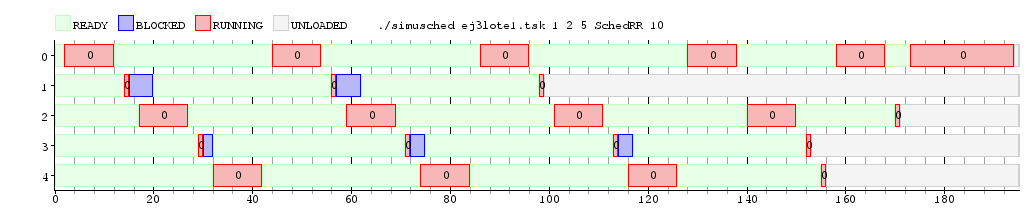
\includegraphics[width=450pt]{./EJ4_RR/ejercicio4-1nucleo.png}
	{$Lote 1$ - Scheduler RR - 1 core}	
 
\end{center}


\indent Con esta simulación, trabajamos con 2 ticks de cambio de contexto.\\
\\
\indent Se puede observar el cambio de tareas cíclico tanto porque terminaron su quantum o porque se bloquearon.\\

\begin{center}
  	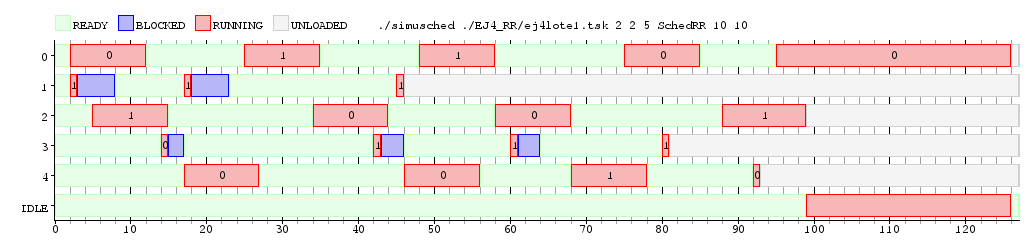
\includegraphics[width=450pt]{./EJ4_RR/ejercicio4-2nucleo.png}
	  {$Lote 1$ - Scheduler RR - 2 core}	
\end{center}

\begin{center}
  	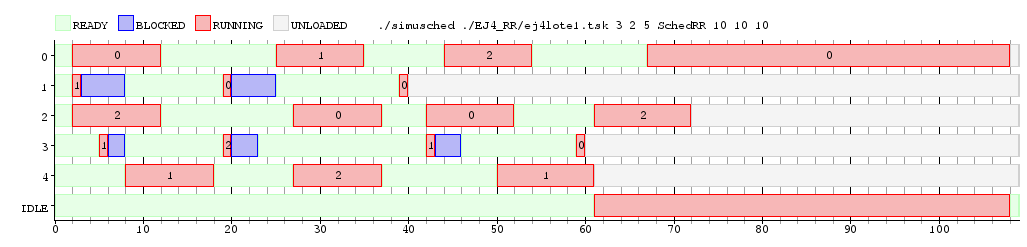
\includegraphics[width=450pt]{./EJ4_RR/ejercicio4-3nucleo.png}
	  {$Lote 1$ - Scheduler RR - 3 core}	
\end{center}

\indent Es notorio, ademas del la ejecuciòn circular de las tareas, un cierto paralelismo al estar trabajando con
2 o 3 cores.\\

\indent Luego, de esta simulación probamos con un lote con tareas que se bloqueen por más tiempo:
 \begin{verbatim}
                                     TaskCPU 70
                                     TaskConsola 5 6 7
                                     TaskCPU 40
                                     TaskConsola 10 9 8
                                     TaskCPU 30
 \end{verbatim}

\indent Manteniendo la misma cantidad de tick para cambio de contexto y core. También, nos parecio prudente, mantener
los mismos valores de $quantum$ obteniendo los siguientes gráficos:

\begin{center}
    	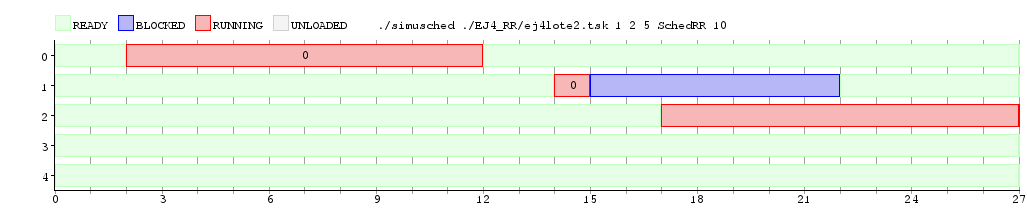
\includegraphics[width=450pt]{./EJ4_RR/ejercicio4-2lote1nucleo.png}
	{$Lote 2$ - Scheduler RR - 1 core}	
 \end{center}

 \begin{center}
    	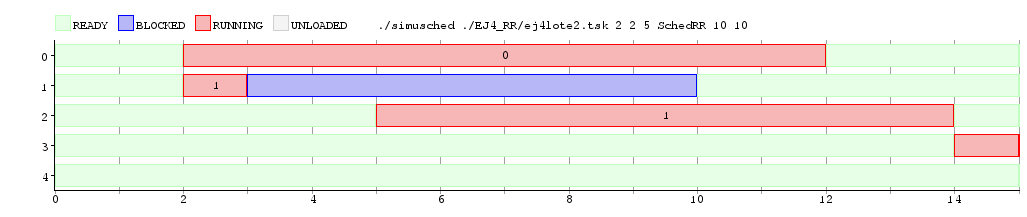
\includegraphics[width=450pt]{./EJ4_RR/ejercicio4-2lote2nucleo.png}
	{$Lote 2$ - Scheduler RR - 2 core}	
 \end{center}
 
 \begin{center}
    	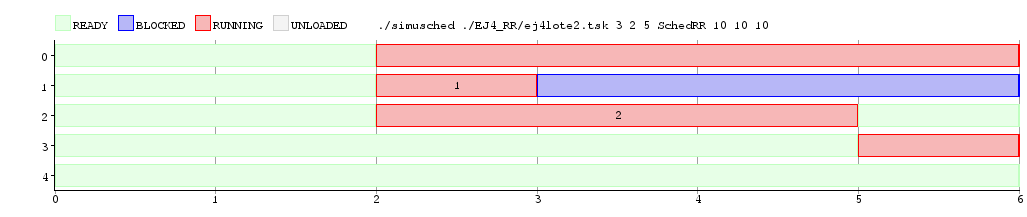
\includegraphics[width=450pt]{./EJ4_RR/ejercicio4-2lote3nucleo.png}
	{$Lote 2$ - Scheduler RR - 3 core}	
 \end{center}

 \indent Con este lote, además de lo observado anteriormente pudimos ver que, al tener una tarea bloqueada
 por un largo tiempo, el scheduler directamente la ignora.\\
 
\indent Luego de estos experimentos pudimos observar ciertos puntos del comportamiento del Round-Robin:\\
\begin{itemize}
\item  Carácter circular del algoritmo.
\item  Desalojo de las tareas cuando se bloquean o terminan y la inmediata asignación del núcleo a la siguiente tarea en caso de existir alguna.
\item  Libre de inanición.
\item  Una tarea bloqueada es ignorada por el scheduler hasta que se desbloquee.
\end{itemize}

\indent Finalmente, dado su carácter circular y equitativo, podemos afirmar que todas las tareas que 
estén en condiciones de correr serán ejecutadas y ninguna será negada de tiempo de procesamiento.\\


\subsubsection[Resolución Ejercicio 5]{Ejercicio 5}
\begin{center}
\textbf{PARTE 1}\\ 
\end{center}

\begin{center}
 \textbf{¿Qué problema están intentando resolver los autores?}
\end{center}

En el paper "Scheduling algorithms for multiprogramming
in a hard-real-time environment" los autores están intentando mostrar y resolver un problema que estaba surgiendo en esa época (1973). El uso de computadoras que controlaban y monitoreaban procesos industriales había empezado a incrementarse notablemente. Con esto aparecen los sistemas que tienen un "tiempo crítico" para procesar. Es decir, sistemas en donde el procesamiento estaba sujeto a un tiempo máximo al cual ejecutarse.\\
Por lo tanto necesitaban maximizar la eficiencia del uso del procesamiento, y para eso afirman que eso es posible mediante un algoritmo de schedulling que asegure procesar antes de ese tiempo crítico.\\
Por eso en el paper proponen dos algoritmos que manejan prioridades: prioridades fijas y dinámicas.\\

\begin{center}
 \textbf{¿Por qué introducen el algoritmo de la sección 7?\\¿Qué problema buscan resolver
 con esto?}
\end{center}

En la sección 7 introducen el algoritmo de prioridades dinamicas tratando de resolver un problema que muestra el algoritmo de prioridades fijas descripto en las secciones anteriores.\\
Al tener prioridades fijas, puede ocurrir inanición. Es decir, puede pasar que siempre lleguen tareas con prioridades más altas de las que se están por corriendo o por correr, dejándolas en espera y nunca atendiéndolas.\\
El algoritmo que presenta en esta sección tiene el nombre de "The deadline driven scheduling algorithm", explicando que se trata de un algoritmo que da más prioridad a las tareas en las que su deadline esté mas cercano. \\

\begin{center}
 \textbf{Explicar coloquialmente el significado del teorema 7}
\end{center}

El teorema 7 enuncia lo siguiente:\\

\textbf{For a given set of m task, the deadline driven scheduling algorithm is feasible if
and only if}
\begin{center}
 \[(C_{1}/T_{1})+(C_{2}/T_{2})+......+(C_{m}/T_{m}) \leq 1\]

\end{center}

Dicho teorema habla sobre la factibilidad y uso de las tareas en el algoritmo que 
se utilice como solución a la particular dificultad del algoritmo del scheduler fixed. \\
Puntualmente el lote de tareas m deberá cumplir una precondición en donde la 
suma de cada una de las relaciones entre el run time o tiempo de ejecución de la tarea, sobre el período de 
la misma de todas las tareas sea igual o menor a 1.\\

Esto quiere decir que el tiempo de ejecución de una tarea deberá ser considerablemente
menor al período de la misma para que el desarrollo y comportamiento del scheduler sea el deseado
y pudiese resolver la dificultad que se había generado por el anterior.\\

\begin{center}
 
\textbf{PARTE 2}\\

\end{center}
\hspace{3pt}
\begin{center}
\textbf{Algoritmo Scheduler Fixed - Explicación de Implementación}\\ 
\end{center}





Luego del estudio del Paper solicitado se realizo la implementación del dicho algoritmo,
utilizando una serie de estructuras para que este funcione acorde a lo pedido:

\begin{itemize}
 \item Un struct denominado  \textbf{tarea} el cual contiene el pid, el run\_time\_actual, periodo dandonos
 informacion de la tarea cargada.
 \item Una lista de $tarea$ nombrada \textbf{tareas}, esta es ordenada segun el periodo de las tareas
 de menor a mayor, obteniendo la prioridad del algoritmo.
  \item Una variable global \textbf{primera\_pasada} con la cual podemos realizar nuestra primer 
 comparacion de periodos entre tareas.
\end{itemize}

Ademas de estas estructuras utilizamos una funcion privada \textbf{insertarOrdenado} la cual como el
nombre lo dice va guardando en nuestra lista de tareas, las tareas a corde se van cargando en su
respectivo lugar comparando los periodos de las mismas.\\
De esta forma, la secuencia del algoritmo fue la siguiente:

\begin{enumerate}
 \item Llega una nueva tarea se la carga e inserta ordenadamente en la lista.
 \item La tarea corre hasta finalizar.
 \item Una vez que finaliza se chequea en la lista cual es la primera en orden de prioridad queda
 esta ready para correr.
 \end{enumerate}

De esta forma, con las estructuras y funciones logramos que nuestro scheduler trabaje de la forma
deseada.\\

Vale aclarar que, para que el scheduler funcione correctamente, es recomendable que los lotes de tareas
cumplan la factibilidad enunciada en el paper estudiado.\\


\hspace{3pt}
\begin{center}
\textbf{Algoritmo Scheduler Dynamic - Explicación de Implementación}\\ 
\end{center}

Una vez finalizado el estudio del paper, y habiendo notado las dificultades puntuales que enuncia el mismo
sobre el anterior Scheduler, se solicito desarrollar uno nuevo que solucione dichos problemas.\\

Para el desarrollo del mismo trabajamos con ciertas estructuras puntuales, las cuales enunciamos
a continuación:\\

\begin{itemize}
 \item Un struct denominado\textbf{tarea}  el cual contiene el pid, el run\_time\_actual, periodo y el deadline para tener
 informacion de la tarea cargada.
 \item Una lista de $tarea$ nombrada \textbf{tareas}, esta es ordenada segun el deadline de las tareas
 de menor a mayor, obteniendo la prioridad del algoritmo.
  \item Una variable global \textbf{primera\_pasada} con la cual podemos realizar nuestra primer 
 comparacion de periodos entre tareas.
\end{itemize}

Además de estas estructuras puntuales, definimos unas funciones de forma privada para poder
desarrollar el Scheduler en cuestión:

\begin{itemize}
 \item Función \textbf{insertarOrdenado}  
 \item Función  \textbf{chequearPeriodos}
  \end{itemize}
  
La función \textbf{insertarOrdenado}  como el nombre lo dice va guardando en nuestra lista $tareas$ las tareas
acorde van siendo cargadas respetando un orden, dicho orden se basa en la prioridad dada por los
deadline de las tareas. A menor deadline la tarea quedara en los primeros lugares de la lista.\\

La función \textbf{chequearPeriodos}, la cual revisa si la tarea que se encuentra al principio de la lista
tiene su deadline menor o igual a cero.\\

A partir de estas estructuras y funciones procedemos a explicar la secuencia de nuestro algoritmo:

\begin{enumerate}
 \item Llega una nueva tarea, se chequea si es la primera en llegar y en caso de no serlo se la inserta ordenadamente.
 \item Empieza a correr una tarea, y en cada Tick de reloj del cpu se va disminuyendo en uno el periodo y deadline
 de todas las demas tareas que no estan corriendo, mientras que la que se encuentra ejecutando
 se le disminuye en uno su run\_time y su periodo.
 \item En caso de que nuestra función booleana $chequearPeriodos$ de True en un tick de reloj
 y la tarea que este corriendo no haya finalizado esta sera desalojada guardando su run\_time actual y su deadline
 insertandola ordenadamente en la lista para que luego pueda finalizar su ejecución.
 \item Si $chequearPeriodos$ no dio nunca True durante la ejecución de la tarea, esta podra finalizar sin
 inconvenientes y posteriormente se cargará la primer tarea de la lista en orden de prioridad.
\end{enumerate}

De esta forma, nuestro Scheduler continua hasta finalizar todas las tareas manteniendo esta secuencia.\\

Vale aclarar, como en el anterior algoritmo, que para un correcto funcionamiento de nuestro
Scheduler es recomendable que el lote de tareas a utilizar cumpla la factibilidad enunciada
en el paper.\\

\newpage

%%%%%%%%%%%%%%%%%%%%%%%%%%%%%%%%%%%%%%%%%%%%%%%%%%%%%%%%%%%%%%%%%%%%%%%%%%%%%%%
%% Conclusión                                                                %%
%%%%%%%%%%%%%%%%%%%%%%%%%%%%%%%%%%%%%%%%%%%%%%%%%%%%%%%%%%%%%%%%%%%%%%%%%%%%%%%

\newpage
\section{Bibliografía}

\begin{itemize}
 \item Cátedra de Sistemas Operativos - Clases teóricas y prácticas (1º Cuatrimestre 2015)
 \item The Little Book of Semaphores
\end{itemize}

\end{document}
